\documentclass[conference]{IEEEtran}
\IEEEoverridecommandlockouts
% The preceding line is only needed to identify funding in the first footnote. If that is unneeded, please comment it out.
\usepackage{cite}
\usepackage{amsmath,amssymb,amsfonts}
\usepackage{algorithmic}
\usepackage{graphicx}
\usepackage{textcomp}
\usepackage{xcolor}
\usepackage{url}
\usepackage{listings}
\lstset{basicstyle=\ttfamily,
  showstringspaces=false,
  commentstyle=\color{red},
  keywordstyle=\color{blue}
}

\lstdefinelanguage{Kotlin}{
  comment=[l]{//},
  commentstyle={\color[HTML]{629755}\ttfamily},
  emph={value, onValueChange, modifier, topBar, horizontalAlignment, vertical},
  emphstyle={\color[HTML]{467CDA}},
  identifierstyle=\color{black},
  keywords={!in, !is, abstract, actual, annotation, as, as?, break, by, catch, class, companion, const, constructor, continue, crossinline, data, delegate, do, dynamic, else, enum, expect, external, false, field, file, final, finally, for, FROM, fun, get, if, import, in, infix, init, inline, inner, interface, internal, is, lateinit, noinline, null, object, open, operator, out, override, package, param, private, property, protected, public, receiveris, reified, return, return@, sealed, SELECT, set, setparam, super, suspend, tailrec, this, throw, true, try, typealias, typeof, val, var, vararg, when, where, while},
  keywordstyle={\color[HTML]{CC7832}},
  morecomment=[s]{/*}{*/},
  morestring=[b]",
  morestring=[s]{"""*}{*"""},
  ndkeywords={@Deprecated, @Composable, @Query, @Insert, @Dao, OnConflictStrategy},
  ndkeywordstyle={\color[HTML]{BBB529}},
  sensitive=true,
  stringstyle={\color[HTML]{6A8759}\ttfamily},
  classoffset=2,
  morekeywords={padding, verticalScroll, items, NavHost, composable, fillMaxSize},
  keywordstyle={\color[HTML]{FFC66D}\itshape},
  classoffset=3,
  morekeywords={REPLACE, CenterHorizontally},
  keywordstyle={\color[HTML]{9876AA}}
}


\def\BibTeX{{\rm B\kern-.05em{\sc i\kern-.025em b}\kern-.08em
    T\kern-.1667em\lower.7ex\hbox{E}\kern-.125emX}}

\begin{document}

\title{Real-time data processing with Apache Kafka}

\author{
    \IEEEauthorblockN{Tobias Fischer, BSc}
    \IEEEauthorblockA{
        University of Applied Sciences Upper Austria \\
        Faculty for Informatics, Communications and Media\\
        Department for Smart and Interconnected Living\\
        Master's program in Mobile Computing \\
        4232 Hagenberg, Austria\\
        tobias.fischer@fh-hagenberg.at
    }
}

\maketitle

\begin{abstract}
Apache Kafka is an open-source distributed stream processing platform commonly used for high-performance data pipelines, streaming analytics, and event-driven applications. This paper provides a comprehensive overview of Kafka, covering key concepts, features, use cases, APIs and architecture. In addition, the integration of Kafka with MQTT for IoT applications is explored, accompanied by a practical implementation of real-time energy data streaming. This real-world example effectively demonstrates the practical application of Kafka in the field of IoT-driven solutions. Finally, the possibilities and limitations of Apache Kafka were discussed and an insight was given into when this powerful event streaming platform should and should not be used.

\end{abstract}

% https://books.google.at/books?hl=de&lr=&id=NMtMEAAAQBAJ&oi=fnd&pg=PP1&dq=kafka+architecture&ots=HZOImWiCQc&sig=WcHcsZasRYxgFq_y31z4mMgWZzI#v=onepage&q=kafka%20architecture&f=false
% Chapter: Meet Kafka

\section{Introduction}
\label{cha:introduction}

In today's dynamic and data-driven world, the ability to process and analyze energy data in real time is becoming increasingly important to optimize energy consumption, improve grid stability and make informed decisions. The benefit of this paper is to explain Kafka in more detail and explain how to set it up using a practical example.

Apache Kafka is a high-performance, distributed event streaming platform developed by the Apache Software Foundation as open source. It was written in Java and Scala and is designed to process large amounts of real-time data with high throughput and low latency. Kafka's key features include fault tolerance, scalability, data integrity and its open source nature, making it a popular choice for a variety of applications, including real-time analytics, data integration and microservice architecture \cite{kafkaDoc}.
\section{Event Streaming}
\label{cha:event-streaming}

Event streaming is a method for processing, transmitting and storing data in real time. Data is viewed here as continuous streams of events \cite{barga2006consistent}.

At its core, event streaming involves the continuous collection and processing of data from various sources, including databases, sensors, mobile devices, cloud services and software applications. This data is organized into a stream of events, which are then stored, processed and analyzed in real time or retrospectively. Event streams can also be forwarded to different target technologies as required. This approach ensures that information is constantly flowing and interpreted so that the right data is available to the right applications at the right time \cite{kafkaDoc}.

\subsection{Apache Kafka as event streaming platform}

Apache Kafka is an open-source distributed event streaming system used for stream processing, real-time data pipelines, and data integration at scale. Kafka combines three key functions for event streaming \cite{kafkaDoc}:

\begin{itemize}
    \item Publish (write) and subscribe (read) to event streams 
    \item Store Streams
    \item Process Streams
\end{itemize}
\section{Functionality}
\label{cha:functionality}

The architecture of Kafka consists of several \textbf{servers} and \textbf{clients}. Kafka uses TCP for communication and can be used on any hardware \cite{kafkaDoc}.

Kafka operates as a distributed cluster of \textbf{servers} that can span multiple data centers or cloud platforms. Brokers manage the data storage layer, while Kafka Connect facilitates seamless data exchange between Kafka and other systems. Kafka clusters are designed for mission-critical applications, offering exceptional scalability, fault tolerance, and data integrity \cite{kafkaDoc}.

Kafka \textbf{clients} enable the development of distributed applications and microservices that process event streams efficiently across multiple machines and are resilient to network disruptions or hardware failures. Kafka has built-in clients that are supplemented by an extensive ecosystem of clients provided by the Kafka community. These clients are available for various programming languages, including Java, Scala, Go, Python, C/C++ and even REST APIs \cite{kafkaDoc}.

\subsection{Main Concepts and Terminology}

The central concept of Kafka is the \textbf{event}. Events are notifications that something noteworthy has occured. Kafka's read and write operations are based on these events. An event consists of a key, a value, a timestamp, and optionally, some metadata headers \cite{kafkaDoc}.

An example event looks like this:

\begin{itemize}
    \item Key: "john.doe@example.com"
    \item Value: "Hello World!"
    \item Timestamp: "01.01.1970 00:00:00"
\end{itemize}

\textbf{Producers} are applications that publish events to Kafka, and \textbf{consumers} are applications that subscribe to and process those events. This decoupled architecture enables Kafka to achieve high scalability, as producers and consumers can operate independently, without the need to wait for each other. This flexibility is further enhanced by Kafka's ability to guarantee data integrity, ensuring that events are processed exactly once \cite{kafkaDoc}.

Events are organized and persistently stored within \textbf{topics}. A topic is more or less similar to a folder in a filesystem, with events acting as the files within that folder. For instance, a topic could be named "measurements". Kafka topics are designed to support multiple producers and consumers: a topic can have any number of producers writing events to it, and any number of consumers subscribing to those events. Events within a topic can be read as many times as necessary. Unlike traditional messaging systems, events are not deleted after consumption. Instead, you configure Kafka to retain your events for a specified amount of time, and old events will be discarded after that period. Kafka's performance remains consistent regardless of data size, making it suitable for long-term data storage \cite{kafkaDoc}.

As illustrated in Figure \ref{fig:partitions}, to enhance scalability and parallelism, Kafka \textbf{partitions} topics into multiple "buckets" distributed across different brokers. This allows multiple consumers and producers to read and write the topic simultaneously to take advantage of the distributed nature of the Kafka cluster. When a new event is published to a topic, it is appended to one of the corresponding partitions. Additionally, events with the same key are written to the same partition, ensuring data consistency and enabling efficient retrieval based on the key. Kafka maintains the order of events within each partition, ensuring that messages are read in the same sequence they were stored \cite{kafkaDoc}.

\begin{figure}[ht]
    \centering
    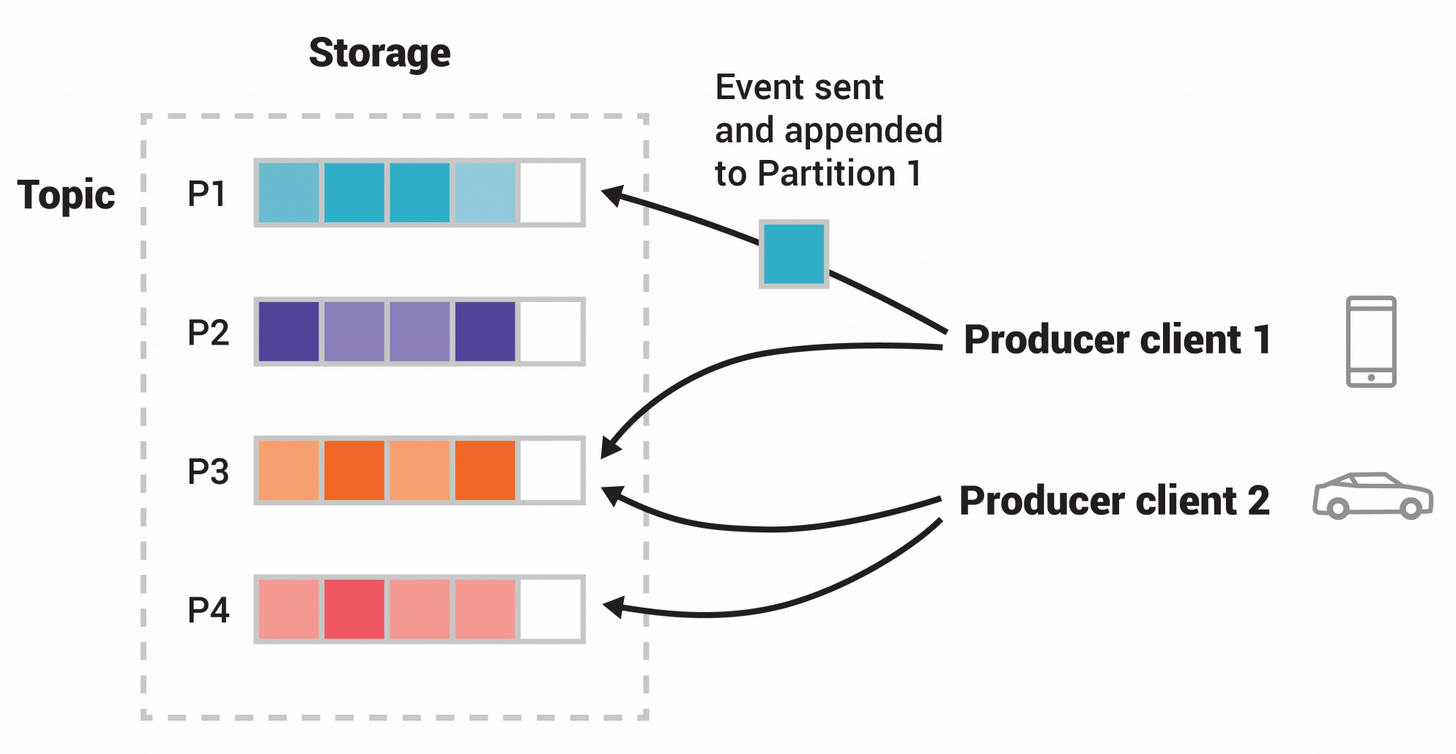
\includegraphics[width=8.5cm]{images/partitions.png}
    \caption{This topic consists of four partitions (P1-P4). Two producers are independently publishing events to the topic, with events with similar keys being grouped into the same partition. Both producers may write to the same partition if necessary \cite{kafkaDoc}.}
    \label{fig:partitions}
\end{figure}

To ensure that data remains accessible even if a broker fails or requires maintenance, each topic can be \textbf{replicated} across multiple brokers. The replication factor of 3 is a common setting that helps to maintain data availability and fault tolerance. Each partition has a partition leader that processes all read and write requests for this partition. The followers of the partition replicate the leader. If the leader fails, a follower becomes the new leader. The leaders are evenly distributed across the cluster, which means that each broker is the leader of several partitions \cite{kafkaDoc}.

\subsection{Architectural Overview}

Figure \ref{fig:architecture} provides a comprehensive overview of the architecture and functionality of Kafka. A major change in the latest versions is the introduction of KRaft as a consensus protocol, replacing Apache ZooKeeper. This change enables Kafka to manage its metadata independently, eliminating the need for external coordination. As a result, Kafka gains self-sufficiency and increased resilience while benefiting from improved scalability and performance \cite{kull2023secure}.

\begin{figure}[ht]
    \centering
    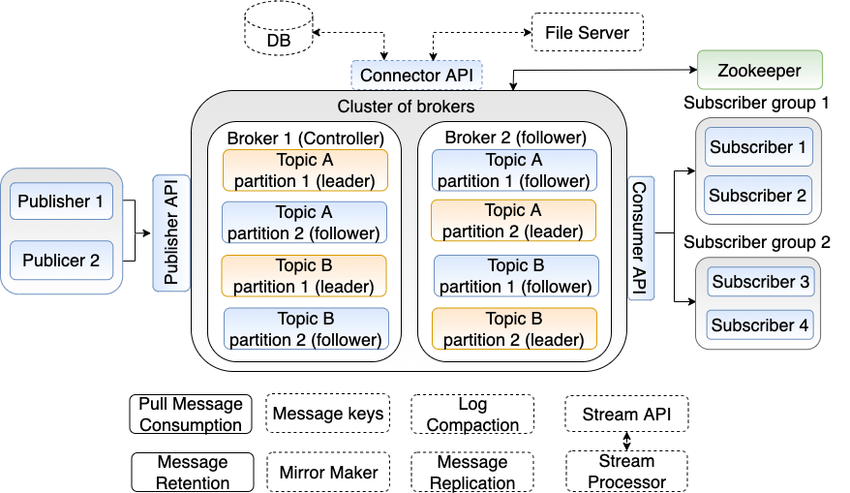
\includegraphics[width=8.5cm]{images/architecture.png}
    \caption{Apache Kafka architecture with mandatory and optional services \cite{lazidis2022publish}.}
    \label{fig:architecture}
\end{figure}
\section{Use Cases}
\label{cha:use-cases}

Kafka offers a wide range of use cases, as highlighted in the official documentation \cite{kafkaDoc}. These include messaging, website activity tracking, metrics, log aggregation, stream processing, event sourcing, and commit log. 

This paper specifically explores the application of Kafka in energy data exchange. The test setup involves a common Austrian Smart Meter equipped with a Smart Meter Adapter from Österreichs Energie. This adapter efficiently transmits data via MQTT, HTTP, and Modbus. The measurement data extracted from the Smart Meter is then streamed using Kafka, as further detailed in Chapter \ref{cha:practical}.
\section{Kafka APIs}
\label{cha:api}

The functionality of Kafka is provided via a language-independent protocol, with clients available for many programming languages. The main Kafka project only maintains the Java clients, the others are available as part of other independent open source projects \cite{shapira2021kafka}. Therefore, Kotlin, which runs on the Java Virtual Machine (JVM), was used for the practical example in this paper. Java can be used from Kotlin and vice versa.

Kafka comprises five core APIs \cite{shapira2021kafka}:

\begin{enumerate}
    \item Producer API: Send data streams to Kafka topics.
    \item Consumer API: Read data streams from Kafka topics.
    \item Streams API: Transform data streams from one topic to another.
    \item Connect API: Build connectors for data transfer between Kafka and external systems.
    \item Admin API: Manage and monitor Kafka cluster components.
\end{enumerate}
\section{MQTT}
\label{cha:mqtt}

MQTT (Message Queuing Telemetry Transport) and Kafka are two essential technologies for managing IoT data. MQTT is a lightweight messaging protocol that is ideal for resource-constrained devices and low-bandwidth networks. Kafka, on the other hand, is a distributed streaming platform that is optimized for high throughput, fault tolerance, and scalability \cite{hugo2020bridging}.

MQTT uses a publish-subscribe model, which makes it easy for devices to share data with each other and with a central service. MQTT messages tend to be small, which minimizes the amount of data that needs to be transmitted over the network. This is important for IoT devices that operate with limited bandwidth \cite{al2020investigating}.

MQTT also emphasizes low latency, which ensures that messages are delivered quickly and reliably. This is important for applications that need real-time data insights \cite{al2020investigating}.

Kafka provides high throughput, which makes it a good choice for processing large volumes of data. It also has fault tolerance features, which ensure that data is not lost in the event of a server outage. Kafka is also scalable, which means that it can be easily expanded to accommodate increasing data volumes \cite{shapira2021kafka}.

When used together, MQTT and Kafka provide a powerful and flexible solution for managing IoT data. MQTT handles the initial data ingestion, while Kafka handles the processing and analysis of the data. This allows for efficient and scalable data management for IoT applications \cite{hugo2020bridging}.
\section{Practical Example}
\label{cha:practical}

This practical example provides a hands-on introduction to the core functionality of Apache Kafka. It demonstrates a simplified scenario to showcase the essential aspects of Kafka's data streaming capabilities. The commands used in this paper apply to Linux; they may differ for other operating systems.

\subsection{Smart Meter}

An EU regulation from the "Clean Energy Package" dictates that 80 \% of households should be equipped with smart meters by 2020. Austrian law requires that 95 \% should be equipped by 2024. Smart meters replace the previous mechanical meters, the Ferraris meters \cite{smartMeterOE}.

The fully electronic smart meters measure energy consumption and power over specific time intervals (e.g. 15 minutes). The measured values are forwarded to the respective grid operators the next day \cite{smartMeterOE}.

A smart meter offers the following new functions: Remote reading by the grid operator, display of consumption values on a display, customer interface, disconnection device and measurement of both energy consumption and energy generation \cite{smartMeterOE}.

\subsubsection{Customer Interface}
All smart meters have a customer interface. With the help of this interface, customers can read detailed consumption and generation information directly from the meter in near real time. The time period in which the data can be read out depends on the manufacturer; in the case of Netz OÖ GmbH's meter, for example, the data is output every second \cite{kernitzkyimehrwert}.

\subsubsection{Smart Meter Adapter}
In Austria, different types of smart meter devices are used by the grid operators. As a result, there are different types of customer interfaces. The Austrian energy industry interest group "Oesterreichs Energie" (\url{https://oesterreichsenergie.at}) has developed a concept for a standardized smart meter adapter that uniforms the provision of data. Therefore it is possible to read the real-time energy data from all smart meters of Austria. The measurement data from this adapter can be queried via MQTT, REST and Modbus TCP. The output format is in JSON and consists of some metadata such as a name defined in the web interface and the measured values with OBIS code and a timestamp \cite{smartMeterAdapter}.

\paragraph{OBIS codes}
The content of the energy measurement data is defined by the IEC 62056-61 standard, which uses a system called OBIS (Object Identification System). The logical OBIS names are represented as a six-character string that corresponds to this OBIS standard. Each data element used in energy meters is uniquely identified by this approach. The complete list of OBIS codes is available on the DLMS Users Association website in the form of a comprehensive Excel file \cite{amaro2011implementing}.

\subsection{Goal}

As more and more IoT (Internet of Things) devices are being used, the amount of data they generate is growing rapidly. In this example, a smart meter adapter is used, but the same ideas can be applied to any IoT device.

To get the data from the smart meter adapter, a local device needs to connect to it via an MQTT broker. This local device could be a Raspberry Pi or another computer running JVM (Java Virtual Machine), MQTT and Kafka. The local device must be connected to the same MQTT broker to which the smart meter adapter is connected, and it must also subscribe to the specific topic to which the smart meter adapter sends its data. In this case, the MQTT broker is also served by the local device.

For a large-scale application, it may not be sufficient to use MQTT alone, so additional streaming functionality is required. The measured values of the smart meter should therefore be streamed via Kafka. In addition to the local device, a Kafka server is needed to process the data and store it for further use. Finally, the energy data can be shared between different services and applications. An illustrative use case could be the forwarding of the data to an energy service provider or the visualization of the data in a mobile app. 

\subsection{Setup MQTT}

First of all, the MQTT broker must be set up on the local device. In this example, Eclipse Mosquitto \cite{mosquitto} was used as the open source MQTT broker.

\subsubsection{Install Eclipse Mosquitto} The following command can be used to install Mosquitto for Debian-based systems:

\begin{lstlisting}[language=bash]
$ sudo apt-get install mosquitto
\end{lstlisting}

\subsubsection{Create config file} The MQTT broker requires a configuration file in order to start properly. This file specifies that it should start with default MQTT port 1883 and allow anonymous access. Mosquitto also supports authentication with username and password, but this is not necessary in this case \cite{mosquitto}. The configuration file named \lstinline{mosquitto.conf} looks like this:

\begin{lstlisting}
listener 1883
allow_anonymous true
\end{lstlisting}

\subsubsection{Start MQTT broker} In Mosquitto, the configuration file can be specified with the \lstinline{-c} option. Therefore, the broker is started with the following command:

\begin{lstlisting}[language=bash]
$ mosquitto -c mosquitto.conf
\end{lstlisting}

\subsection{Connect Smart Meter Adapter}

After starting the broker, the smart meter adapter must send its data to a specific topic. As shown in Figure \ref{fig:sma}, several parameters must be entered. Firstly, the protocol must be determined. As the configured broker does not support encrypted connections, \lstinline{TCP-mqtt} is used. The host name of the local device must be entered in the Broker field, in this case \lstinline{192.168.68.31}. As specified in the configuration file, port 1883 is intended for the broker. In addition, a unique client ID is required for MQTT, which ensures a unique assignment to a specific broker. Redundancies are irrelevant, as the system automatically assigns a new ID in such cases. Finally, a topic must be specified in order to subscribe to it later. Specifically, a simple theme called \lstinline{sma} was used.

\begin{figure}[ht]
    \centering
    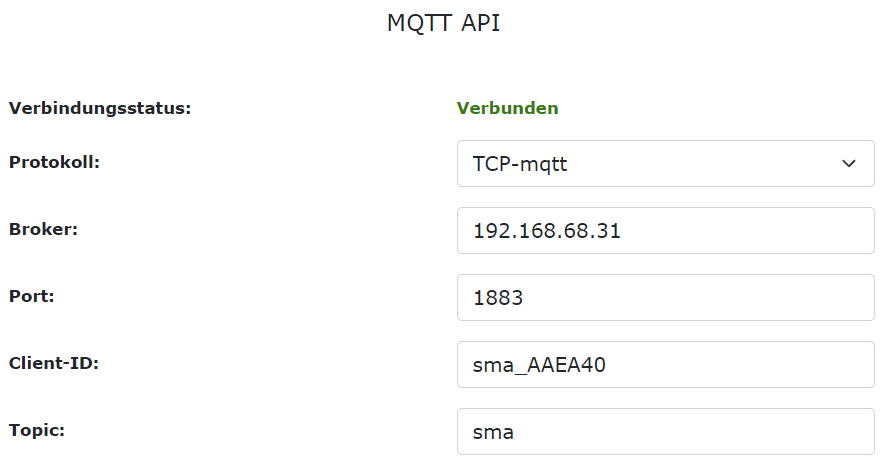
\includegraphics[width=8.5cm]{images/sma.png}
    \caption{MQTT settings of the Smart Meter Adapter.}
    \label{fig:sma}
\end{figure}

\subsection{Setup Kafka}

For demonstration purposes, the local device hosts the Kafka server. In a real-world deployment, however, the Kafka server would be deployed on a remote server or even in a cluster of servers to handle the high volume of data from a large number of smart meters. This enables the application to scale effectively to support a vast network of smart meters.

\subsubsection{Download Apache Kafka} Kafka is available for download in different versions on the official Apache Kafka website: \url{https://kafka.apache.org/downloads}. Once the desired version has been selected, the archive must be downloaded and then unpacked in a suitable location on the system. If the Kafka directory is not contained in the system's PATH environment variable, the following setup commands in this section must be executed within the unpacked Kafka directory.

\subsubsection{Generate a Cluster UUID (Universally Unique ID)} The cluster ID serves as a unique identifier for a Kafka cluster, enabling all nodes within that cluster to recognize each other and collaborate effectively by sharing consistent data and configurations. In this case, a random ID is created, but if there are several instances in the cluster, they must share this ID \cite{shapira2021kafka}. The generation of the ID works as follows:

\begin{lstlisting}[language=bash]
$ KAFKA_CLUSTER_ID=\\
    "$(bin/kafka-storage.sh random-uuid)"
\end{lstlisting}

\subsubsection{Format Log Directories} To ensure proper initialization and readiness of the Kafka data directories for storing new data, it is essential to format the entire data directory, i.e. to capture all partitions, replicas and associated data structures. This comprehensive formatting procedure also deletes all existing data and allows the cluster to reboot, avoiding potential complications due to corrupted or outdated data \cite{shapira2021kafka}. The configuration of the Kafka cluster remains unchanged from the default settings. The formatting process can be performed with the following command:

\begin{lstlisting}[language=bash]
$ bin/kafka-storage.sh format \\
    -t $KAFKA_CLUSTER_ID \\
    -c config/kraft/server.properties
\end{lstlisting}

\subsubsection{Start the Kafka Server} After setting up the cluster, it must be started with KRaft as specified in the next command:

\begin{lstlisting}[language=bash]
$ bin/kafka-server-start.sh \\
    config/kraft/server.properties
\end{lstlisting}

\subsection{Implementation}

With the completion of the initial setup procedures, it is now possible to proceed to the implementation phase of the project. The implementation details of this project are publicly available on GitHub at \url{https://github.com/tformatix/saap-apache-kafka}.

The system is based on a producer-consumer architecture, with the producer running on the local device to collect energy data and the consumer running on another device, e.g. a mobile app, to visualize the data.

\subsubsection{Kafka Producer}

Locally, the \lstinline{SmaMqttConsumer} first subscribes to the MQTT topic \lstinline{sma}, in which the smart meter adapter publishes its measurements. After receiving a measurement, the received JSON is converted into a Kotlin object and forwarded to the \lstinline{SmaKafkaProducer}.

\paragraph{SmaMqttConsumer}

The MQTT consumer uses the package \lstinline{org.eclipse.paho.client.mqttv3}. As MQTT is not the main focus of this paper, it will not be explained further.

\paragraph{SmaKafkaProducer}

The code for the producer class is shown in Figure \ref{fig:producer}. When the class is initialized, a Kafka producer object is created with its properties. These properties include the bootstrap servers, i.e. the initial hosts that the Kafka client uses to find other servers in the cluster \cite{kafkaDoc}. In this example, only one server is running locally, so the bootstrap servers are set to \lstinline{localhost:9092}. Kafka can transmit more than just simple strings, but other objects must be serialized before they can be sent. The serializer and deserializer are responsible for converting objects from one format to another. In this case, the key is simply the name entered in the adapter's web interface and the value is the entire JSON payload. Therefore, only one \lstinline{StringSerializer} is needed.

The \lstinline{produce} method sends a new event to the Kafka stream. A \lstinline{ProducerRecord} object is created that specifies the topic (in this case \lstinline{sma-kafka}) as well as the key and value for the event. Finally, the record is sent to the Kafka cluster.

\begin{figure}[ht]
    \centering
    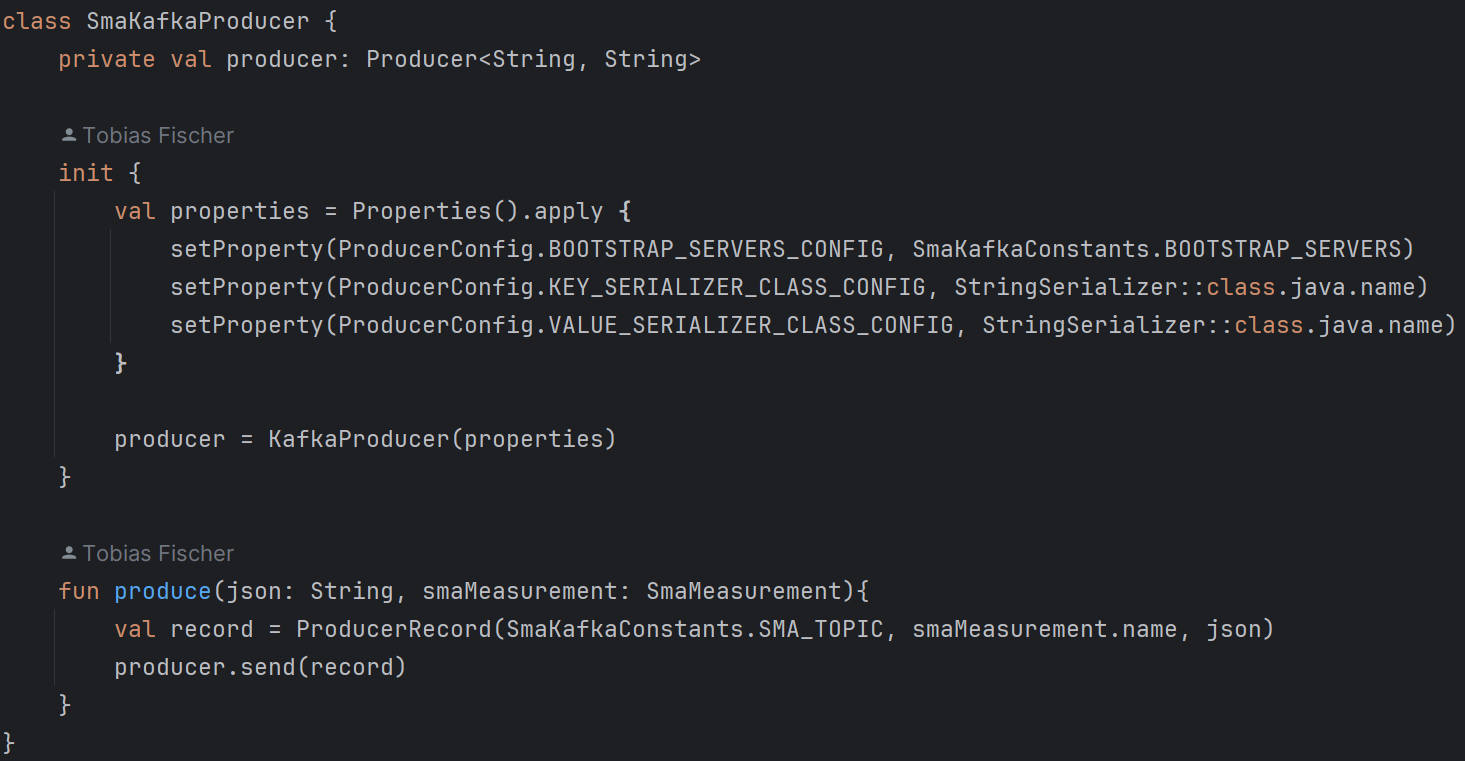
\includegraphics[width=8.5cm]{images/producer.png}
    \caption{SmaKafkaProducer without imports.}
    \label{fig:producer}
\end{figure}

\subsubsection{Kafka Consumer}

In addition to the producer, the \lstinline{SmaKafkaConsumer} class requires two other properties: a group ID and an offset. The implementation of the class can be seen in Figure \ref{fig:consumer}.

Kafka groups consumers in order to distribute the processing load evenly. One or more partitions are assigned to each consumer so that it can concentrate on specific message streams. Within a group, the partitions are distributed among the consumers to avoid overloading a single instance \cite{shapira2021kafka}. In this example, the group ID is generated randomly as there is only one consumer.

The configuration for resetting the automatic offset determines when Kafka starts reading events from the topic. There are two options available: \lstinline{earliest}, which instructs Kafka to start at the beginning of the event stream, and \lstinline{latest}, which restricts Kafka to only process new events \cite{kafkaDoc}. In this case, the \lstinline{earliest} option is used.

The \lstinline{seekToBeginning} method ensures that Kafka retrieves all previously stored events before the consumer starts \cite{kafkaDoc}. The consumer then subscribes to the \lstinline{sma-kafka} topic and enters an infinite loop. Within the loop, the consumer polls for events for one second and then runs through all data records recorded during this time interval.

\begin{figure}[ht]
    \centering
    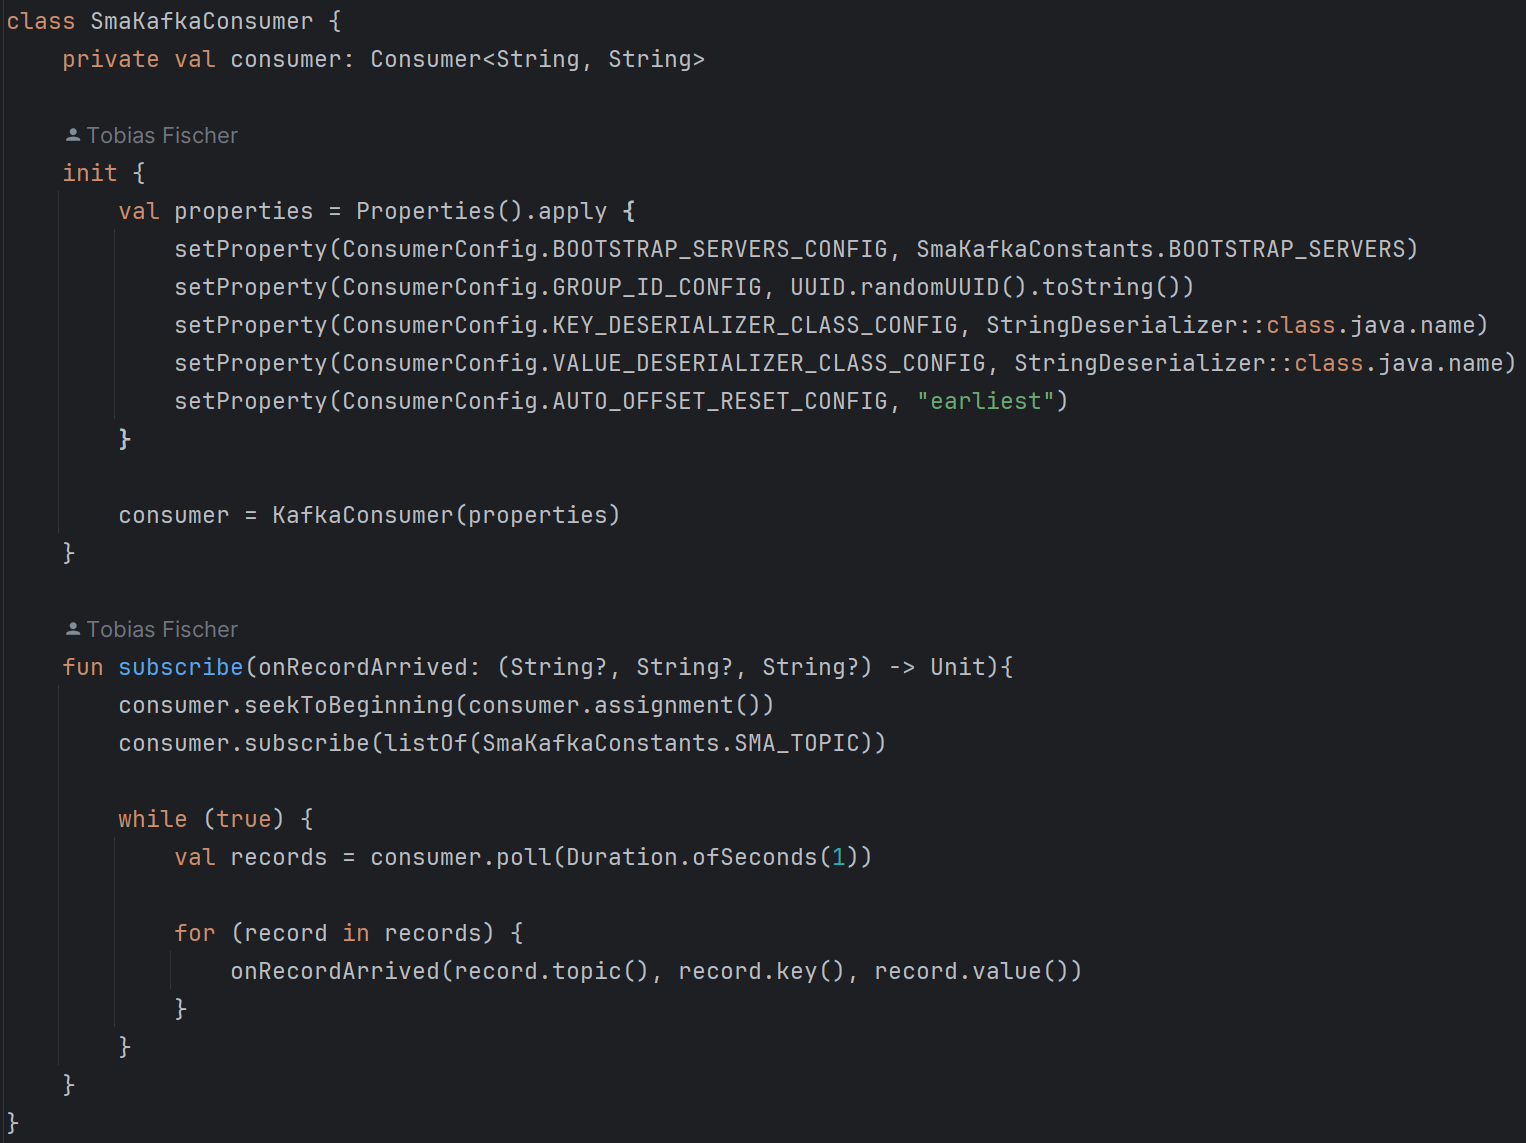
\includegraphics[width=8.5cm]{images/consumer.png}
    \caption{SmaKafkaConsumer without imports.}
    \label{fig:consumer}
\end{figure}

\section{Limitations}
\label{cha:pros_cons}

Kafka offers significant benefits, but it is also important to consider its limitations before adaption.

Kafka's core functionality does not provide comprehensive monitoring capabilities, requiring additional tools or custom implementations. Kafka's append-only nature hinders message modification or deletion after they have been produced. While Kafka offers high throughput and low latency, it may not be ideal for applications demanding sub-millisecond response times due to internal overhead. Kafka's distributed architecture and network reliance make it vulnerable to network disruptions. MQTT may be a better choice for scenarios with large client numbers (tens of thousands) due to its lightweight protocol and efficient handling of many connections.
Kafka is designed for high throughput of small messages; while larger messages are supported, efficiency is maximized with small payloads \cite{Pacheco2023}.

For the specific use case of energy data, storing all data may not be feasible due to privacy concerns. In addition, Kafka is not well suited for this application due to the frequent measurements in network-constrained environments. MQTT would be a better choice for these scenarios as it is optimized for resource-constrained devices. Furthermore, Kafka's extensive fault tolerance overhead for energy data is unnecessary as the loss of a single data point is not significant.
\section{Conclusion}
\label{cha:conclusion}

Kafka is undoubtedly an excellent tool for processing event streaming. However, when it comes to energy data applications, MQTT might prove to be the more suitable choice, especially due to the described limitations of Kafka. Kafka is great for scenarios where numerous servers generate a large amount of logs or other data streams. In cases involving a large network of clients with potentially limited network resources, alternative solutions may prove more viable.

\graphicspath{{images/}}

\bibliographystyle{IEEEtran}
\bibliography{references} % Biblatex-Literaturdatei (references.bib)

\end{document}